% vim:ts=4:sw=4
%
% Copyright (c) 2008-2009 solvethis
% Copyright (c) 2010-2012 Casper Ti. Vector
% Public domain.

\chapter{Overview}
\section{Experimental Setup}
In our work, the OpenHRP 3.0 simulator was used to produce a snap assembly process using HIRO, a simulated 6 DoF dual-arm anthropomorph robot. A CAD derived male and female camera molds with 4 cantilever snaps were used. The male part was rigidly mounted on the robot's wrist while the female part was fixed on the ground. The snap part of this task is a cantilever snap.\\

\begin{figure}[h]
    \centering
    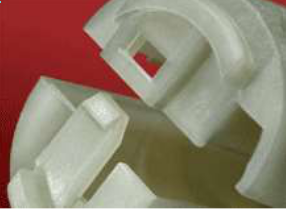
\includegraphics[scale=0.4]{img/cantilever.png}
    \caption{Cantilever Snap}
    \label{snap}
\end{figure}

\indent The Side Approach strategy \cite{2012ICMA-Rojas-PivotApproach} was used to drive the assembly strategy. The Relative Change Based Hierarchical Taxonomy System (RCBHT) was used to aid in the state estimation by encoding force and torque signals in increasingly abstracted ways. Details of this work can be seem in \cite{2013IJMA-Rojas-TwrdsSnapSensing}.
\section{Control Framework}
The control framework used a Control Basis approach \cite{2012JAR-Rojas-AutHetBotAsmbly} in conjunction with the Pivot Approach strategy to produce four intuitive states in the assembly task. Namely, the Approach state, the Rotation state, the Insertion state and the Mating state. In the Approach state, the upper part approaches the lower part. After the Approach state, the Rotation states the upper male part rotates until it meets the lower part and makes contact. The contact will induce a force and moment into the male part's force sensor. If this force surpasses an empirically derived threshold, the strategy will move to the Insertion stage where the assembly force that drives the assembly is increased to insert the upper male part into the lower female part. Here an empirically derived force threshold is used to identify if proper contact is made. If so, the strategy then moves to the Mating state, which ensure that both parts maintain their contact position in a stable manner.\\

\begin{figure}[h]
    \centering
    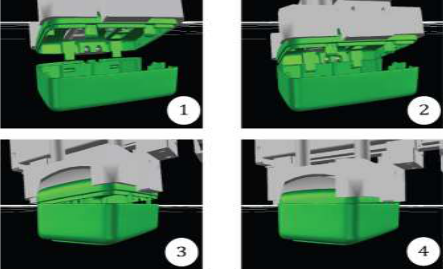
\includegraphics[scale=0.7]{img/controlStrategyFourStep.png}
    \caption{Four control states}
    \label{RCBHT}
\end{figure} 

\section{The Relative Change-Based Hierarchical Taxonomy (RCBHT)}
The RCBHT is a state estimation technique that abstracts force-torque signatures by hierarchically encoding relative change in contextually sensitive ways. Four increasingly abstracted layers were used to encode the relative change with force signatures. The taxonomy layers are as follows the Primitive layer (P), the Motion Composites layer (MCs), the Low-level Behavior layer (LLBs), and the High-level Behavior (HLBs). A fifth layer can be used as a monitor for state estimation. In this work, the SVM will serve this purpose. The RCBHT layers are shown here \\

\begin{figure}[h]
    \centering
    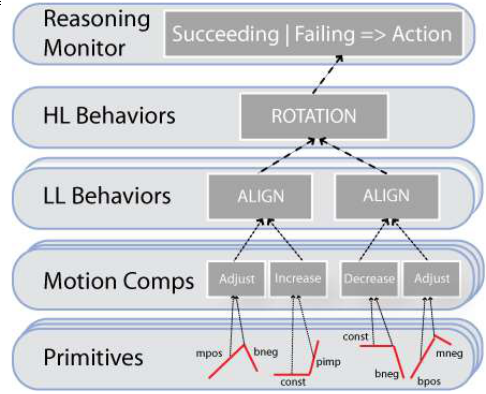
\includegraphics[scale=0.6]{img/fiveLayers.png}
    \caption{Five Layers of RCBHT}
    \label{RCBHT}
\end{figure} 

\indent In our work, we used three lower layers instead the five layers. The details about RCBHT can be seen in \cite{2012IROS-Rojas-RCBHT}. In this section, we will only describe the three lower layers.
\subsection{Primitive layer}
In the primitive layer, linear regression is used to partitioned the force signal into linear segments. Each segment is classified into one of nine labels according to the gradient. The upper layers are based on Primitive layer labels.
\subsection{Motion Composites layer}
Motion Composites (MCs) labels consist of: adjustment, increase, decrease, constact, positive contact, negative contact, and unstable motions followed by a protocol, which looks for matching pair of Primitive labels. The protocol is not only used to produce MC labels, but also for minimizing the effects of noise or erroneous primitive segments. The protocol can be seem in \ref{fig:MotionCompositions} in Appendix. 
\subsection{Low-level Behavior layer}
Low-level Behaviors are derived by looking for specific MC pairs, which highly abstracts the F/T information. The set consist of: {push, 'PS'}, {pull, 'PS'}, {contact, 'CT'}, {fixed, 'FX'}, {alignment, 'ALIGN'}, {shift, 'SH'}, and {noise, 'N'}. \\

\indent Details about RCBHT can be seen in appendix.


